\documentclass[10pt,a4paper]{article}
\usepackage[utf8]{inputenc}
\usepackage[italian]{babel}
\usepackage{amsmath}
\usepackage{amsfonts}
\usepackage{amssymb}
\usepackage{graphicx}
\usepackage{gensymb}
\usepackage[left=2cm,right=2cm,top=2cm,bottom=2cm]{geometry}
\newcommand{\rem}[1]{[\emph{#1}]}

\author{Gruppo BN \\Lisa Bedini,  Federico Belliardo, Marco Costa}
\title{Esperienza 13: Semaforo}

\begin{document}
\maketitle

%TODO - Secondo me in tutta la relazione le immagini non sono il massimo avrei voluto mettere le immagini del flip-flop congelato, ma non le abbiamo prese. Le immagini che mostrano le misure dei tempi non sono il massimo. Io le toglierei.

\section{Scopo dell'esperienza}
Lo scopo dell'esperienza � di realizzare un semaforo come macchina a stati finiti tale che
\begin{itemize}
\item nello stato ENABLED esegua un ciclo in cui si abbiano accesi (per la durata di un colpo di clock e nel seguente ordine) Led verde, Led verde e giallo, Led rosso.
\item nello stato NOT ENABLED faccia lampeggiare il Led giallo (sincronamente  col clock).
\end{itemize}
Il semaforo va realizzato sia tramite circuiti integrati, sia programmando Arduino.

\section{Materiale a disposizione}
%correggi
\begin{itemize}
\item 2 SN7474 Dual D-FlipFlop
\item 1 SN7400 Quad NAND gate
\item 1 SN708 Quad AND gate
\item 1 7432 Quad OR gate
\item DIP switch
\item 3 Led: verde, giallo, rosso
\end{itemize}
%I valori delle componenti sono state misurate con multimetro digitale (incertezza riportata sul manuale).
%Le differenze di potenziale sono state misurate tramite oscilloscopio, se non indicato diversamente, e come incertezza si � presa la sensibilit� dei cursori pi� il 3\% di calibrazione.
%Per misurare i tempi si � usato l'oscilloscopio e come relativa incertezza si � preso il massimo fra la sensibilit� dei cursori e la semidispersione dei valori plausibili.

\section{Stato Enabled}
%figura circuito con piedini numerati
Per realizzare il solo stato enabled abbiamo optato per una macchina di Moore non essendoci alcun tipo di input. In figura \ref{fig:FSMenabled} abbiamo disegnato le transizioni e la codifica dei vari stati. Abbiamo deciso di usare solo 2 FF in quanto due bit erano sufficienti per codificare i tre stati richiesti. Indicheremo SEMPRE (anche nei punti successivi della relazione) $Q_1$ il bit pi� significativo, mentre $Q_0$ sar� sempre il bit meno significativo della codifica.
\begin{figure}[!htb]
\centering
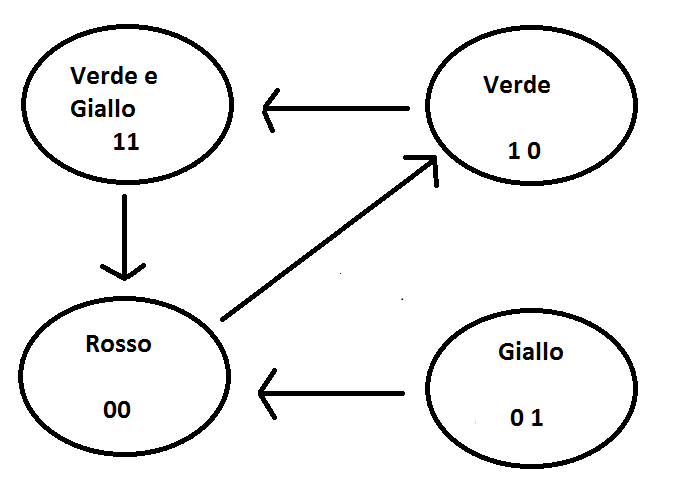
\includegraphics[scale=0.7]{FSMenabled.png}
\caption{Diagramma dello stato Enabled. Le transizioni avvengono aad ogni colpo di clock\label{fig:FSMenabled}}
\end{figure}
%In arrivo ftrase ambigua
Abbiamo codificato gli stati in modo che  i Led verde e giallo siano pilotati da due bit distinti, rispettivamente $Q_1$ e $Q_0$ nel nostro caso. In questo modo ci sar� pi� facile in seguito poter far lampeggiare il solo Led giallo.
Abbiamo deciso di codificare lo stato rimanente (10) come lo stato in cui il solo Led giallo � acceso. Tale stato compare nel circuito solo nella eventualit� in cui i FF si accendano in questo stato. Salvo in questo caso, 01 non compare pi� nei cicli successivi. Le tabelle di transizione sono riportate in tabella \ref{tab:transiozioneenabled}.
\begin{table}[!htb]
\centering
\begin{tabular}{|c|c||c|c||c|c|c|}
\hline
$Q_{1,n}$ & $Q_{0,n}$ & $Q_{1,n+1}$ & $Q_{0,n+1}$ & $LV$ & $LG$ & $LR$\\
\hline
0 & 0 & 1 & 0 & 0 & 0 & 1 \\
0 & 1 & 0 & 0 & 0 & 1 & 0\\
1 & 0 & 1 & 1 & 1 & 0 & 0\\
1 & 1 & 0 & 0 & 1 & 1 & 0\\
\hline
\end{tabular}
\caption{Tabella di verit� della funzione di transizione fra stato $n$ e il successivo $n+1$ dei due D-FF\label{tab:transizioneenabled}}
\end{table}

Con un rapido studio tramite mappe di Karnaugh ci si convince facilmente che ponendo i due don't care\footnote{� lecito assegnare a questi don't care tutte le combinazione tranne 01: in questo caso infatti la macchina resterebbe perpetuamente in questo stato} pari a 0 si ottiene che la funzione richiesta � \begin{equation}
Q_{1, n+1} = \bar{Q}_{0,n}\qquad Q_{0,n+1} = \bar{Q}_{0,n}\cdotQ_{1,n} 
\end{equation}
Cos� si ha che lo stato non richiesto 01 ("solo giallo acceso"), transisce nello stato 00 ("solo rosso acceso").\\
Una volta codificati gli stati, abbiamo assegnato alle uscite $L_V$ (Led Verde), $L_G$ (Led giallo), $L_R$ (Led rosso) i seguenti valori:
\begin{equation}
L_V = Q_1 \qquad L_G = Q_0 \qquad L_R = \bar{Q}_0\cdot \bar{Q}_1
\end{equation}
Questo era in effetti il modo pi� semplice per realizzare i collegamenti fra i FF e le uscite: per come erano stati codificati gli stati, i led verde e giallo sono pilotabili direttamente dal rispettivo bit, mentre per il Led rosso abbiamo scelto l'unica funzione che valga 1 solo sullo stato 00. In effetti avremmo pure potuto prendere come funzione per pilotare il Led rosso $\bar{Q_1}$, a patto per� di avere 01 stato in cui sia il giallo che il rosso sono accesi. Abbiamo preferito usare una porta in pi� qui e avere la possibilit� di controllare il Led giallo direttamente.
% e ce credo, erano davvero una cazzata...
%non mi piace come � scritta questa parte: ad esempio all'inizio dico subito che lo stato 0 1 � il giallo ma solo ora dichiao in effetti a cosa sia collegata l'uscita L_G... Inoltre, sebbne la tabella di transizione la ho scritta bene, devo far capire che poi i q_n+1 sarebbero gli ingressi D...
Abbiamo implementato il circuito come in figura\ref{fig:circenable}.
Abbiamo collegato i clear e reset dei FF a $V_CC$ tramite resistenze di pull-up di resistenza circa $1.5\mbox{k}\Omega$.
Abbiamo collegato i Led a terra tramite resistenza da circa $330\Omega$ per limitare la corrente.  
Abbiamo preso le forme d'onda di Clock e ciascuno dei tre Led tramite oscilloscopio.
%Inserire figure!
Si osservi che i segnali dei Led (e quindi delle uscite dei FF, a meno di ritardi trascurabili) diventano positive quando il clock � sul fronte positivo (abbiamo edge-positive triggered Flip-Flop).
Inoltre, come atteso, si osserva che il Led Giallo e Rosso stnno accesi per un periodo e spenti per i due successivi, mentre il Verde il contrario.

\section{Semaforo completo}
Abbiamo optato di usare una macchina di Mealy per realizzare il semaforo completo. Si � mantenuta la stessa codifica degli stati in termini di bit utilizzata precedentemente. In questo modo la matrice di transizione nello state Enabled � identica a quella precedente. Abbiamo chiamato E il valore logico dell'enable.
Abbiamo deciso di scegliere lo stato Enabled attivo alto (ossia quando $E = 1$):%spiega perch�
In tabella \ref{tab:semaforocompleto} abbiamo la matrice di transizione e i valori delle uscite implementata (i don't care sono stati assegnati)
\begin{table}
\centering
\begin{tabular}{|c||c|c||c|c||c|c|c|}
\hline
$E$ & $Q_{1,n}$ & $Q_{0, n}$ & $Q_{1, n+1}$ & $Q_{0, n+1}$ & $LV$ & $LG$ & $LR$\\
\hline
0 & 0 & 0 & 0 & 1 & 0 & 0 & 0 \\
0 & 0 & 1 & 0 & 0 & 0 & 1 & 0\\
0 & 1 & 0 & 0 & 1 & 1 & 0 & 0\\
0 & 1 & 1 &  0 & 0 & 1 & 1 & 0\\
\hline
1 & 0 & 0 & 1 & 0 & 0 & 0 & 1 \\
1 & 0 & 1 & 0 & 0 & 0 & 1 & 0\\
1 & 1 & 0 & 1 & 1 & 1 & 0 & 0\\
1 & 1 & 1 & 0 & 0 & 1 & 1 & 0\\
\hline
\end{tabular}
\caption{Matrice di transizione e valori di verit� per le uscite nel caso di semaforo completo.\label{tab:semaforocompleto}}
\end{table} 
Nel caso Not Enabled, abbiamo deciso di mantenere lo stato 01 ad essere con solo il Led giallo acceso. Abbiamo deciso di farlo transire verso 10 : in modalit� Enabled lo stato 00 aveva solo il Led rosso acceso, pertanto con una aggiunta di un AND con il bit E si � riusciti a mantenere il circuito gi� montato in precedenza. Le transizioni degli altri stati (10 e 11) sono state scelte in modo che le relative mappe di Karnaugh risultassero le pi� semplici possibili compatibilmente col fatto che gli stati 10 e 11 non devono permanere mai.
Abbiamo cos� ottenuto come funzioni logiche:
\begin{equation}
Q_{0, n+1} = \bar{Q}_{0,n}\cdot(\bar{E}+Q_{1,n})\qquad
Q_{1, n+1} = E\cdot \bar{Q}_{0, n}
\end{equation}
Con lo stesso modo si sono scelte le funzioni di output dei Led relativamente ai soliti stati indesiderati 11 e 10. Stavolta i valori logici degli output sono dei veri don't care. Abbiamo ottenuto le seguenti equazioni:
\begin{equation}
LV = Q_1\qquad LG = Q_0\qquad LR = E\cdot(\bar{Q}_1\cdot\bar{Q}_0)
\end{equation}
Si osservi che non abbiamo alterato le connessioni delle uscite realizzate nel punto precedente, e ci si � limitato ad aggiungere un AND con $E$ in un solo punto.
%in realt� ni: penso di aver aggiuynto uan porta per evitare di effettuare scollegamenti nel punto precedente
Si osservi che in questo caso abbiamo implementato un meccanismo di abilitazione asincrona: non appena si cambia lo stato di $E$, indipendentemente dal fronte del clock, si ha che il semaforo cambia stato di abilitazione. Il Led Rosso � collegato all'enable non tramite altri D-Latch, quindi  se � acceso mentre $E$ passa da 1 a 0, avviene immediatamente il cambio dei valori logici delle uscite previste nel caso di $E = 0$, ossia si passa all'uscita $LG=1$ senza aspettare il clock.
Per le altre uscite non ci sono problemi in quanto sono collegate ad $E$ solo tramite i vecchi D-Latch.
Per realizzare un meccanismo di abilitazione sincrona, ossia per fare in modo che il semaforo registri solo cambiamenti di $E$ che avvengono sul fronte alto del clock, si � collegato $E$ direttamente ad un terzo D-Latch, come in figura\ref{fig:sincrono}.
Si osservi che a differenza di prima, si osserva una transizione diversa se passiamo da Enabled a not Enabled e se ci troviamo nello stato 00 (Led rosso acceso); nel circuito costruito prima si passa subito a stato spento 00, che poi transisce a 01 (ossia con il solo Led Giallo acceso). Adesso si ha una transizione a 10, in cui si ha il Led Verde acceso, e poi si entra nel ciclo 00/01, in cui si ha il Led Giallo lampeggiante.
\section{Semaforo con Arduino}
Adesso vogliamo implementare lo stesso semaforo programmando Arduino. Abbiamo optato per una macchina di tipo Moore, pi� semplice concettualmente da realizzare.
Abbiamo collegato le uscite di Arduino 9, 10, 11 tramite il buffer rispettivamente ai Led Verde, Giallo, Rosso, inserendo resistenza da $330\Omega$ su ciascuno per limitare la corrente.
Queste uscite sono state dichiarate come OUTPUT nel programma utilizzato.
L'enable � stato collegato all'uscita 8, e nel programma � dichiarato come INPUT-PULLUP (ossia alto se interruttore aperto e basso se chiuso).
Dato che con Arduino si hanno in genere un numero di bit a sufficienza, nello scriere il programma abbiamo assegnato ad ogni LED un bit diverso. In questo modo si ha uno stato per ogni LED acceso, pi� lo stato spento e lo stato in cui Verde e Giallo sono accesi. Abbiamo considerato solo i vari stati che ci servono: quelli indesiderati non si presentano mai dato che l'inizializzazione (nello stato in cui tutto � spento) viene fatta da noi nel programma e non casualmente come nel caso dei FF.
Il funzionamento del programma mima il comportamento della macchina a stati finiti precedentemente costruita: legge lo stato in cui si trova attualmente, legge il valore di Enable (attivo alto) e a quel punto decide in che stato finire. Il vantaggio rispetto a prima � che � possibile settare il tempo di permanenza di uno stato in modo indipendente dagli altri. Dopo viene retto il valore di Enable (abilitazione sincrona) e vengono cambiati i valori di output secondo lo stato in cui si trova la macchina (che essendo di tipo Moore, ha ad ogni stato associato un ben definito valore di output)
%spiega meglio l'ordine, anche perch� non � proprio questo l'ordine utilizzato nel programmino  del prof.
\section{Conclusioni}

\end{document}







